\chapter{Projekt aplikacji OffCalendar}
\label{cha:proAppOff}

Po dokonaniu gruntownej analizy technicznej oraz analizy wymagań, należy przystąpić do realizacji drugiego z celów pracy, którym jest budowa aplikacji wspierającej tryb offline.

Tworzonej aplikacji nadano nazwę OffCalendar. Będzie ona umożliwiać użytkownikom zarządzanie wydarzeniami oraz otrzymywanie notyfikacji e-mail o tych zbliżających się. Głównym czynnikiem wyróżniającym OffCalendar od innych aplikacji, zajmujących się zarządzaniem wydarzeniami, ma być pełne wsparcie dla trybu offline oraz synchronizacja pomiędzy wszystkimi urządzeniami na których zalogowany jest dany użytkownik.

W rozdziale tym zostanie opisana architektura aplikacji OffCalendar. Aplikacja składa się z dwóch głównych części: klienckiej oraz serwerowej. Przedstawiony zostanie model komunikacji pomiędzy danymi częściami aplikacji oraz zaprezentowane zostaną najważniejsze ich elementy. W części klienckiej wyszczególnione zostaną założenia lokalnego gromadzenia danych użytkownika, metody komunikacji z częścią serwerową, detekcja i przełączanie pomiędzy trybami offline/online oraz graficzny interfejs użytkownika. W części serwerowej opisana zostanie warstwa danych, interfejsy przeznaczone do komunikacji z częścią kliencką oraz założenia procesu synchronizacji danych pomiędzy częściami aplikacji. Szczególną uwagę zwrócono na bezpieczeństwo komunikacji i danych.

\section{Architektura systemu}
\label{sec:archSys}

Z uwagi na fakt, iż fundamentalna dla aplikacji OffCalendar jest możliwość działania na różnych urządzeniach oraz wspieranie trybu offline, projekt realizowany będzie z wykorzystaniem architektury klient-serwer (rysunek 3.1\footnote{\url{http://www.prideparrot.com/Source-Codes/Images/REST.png}}).

\begin{figure}[H]
\centering
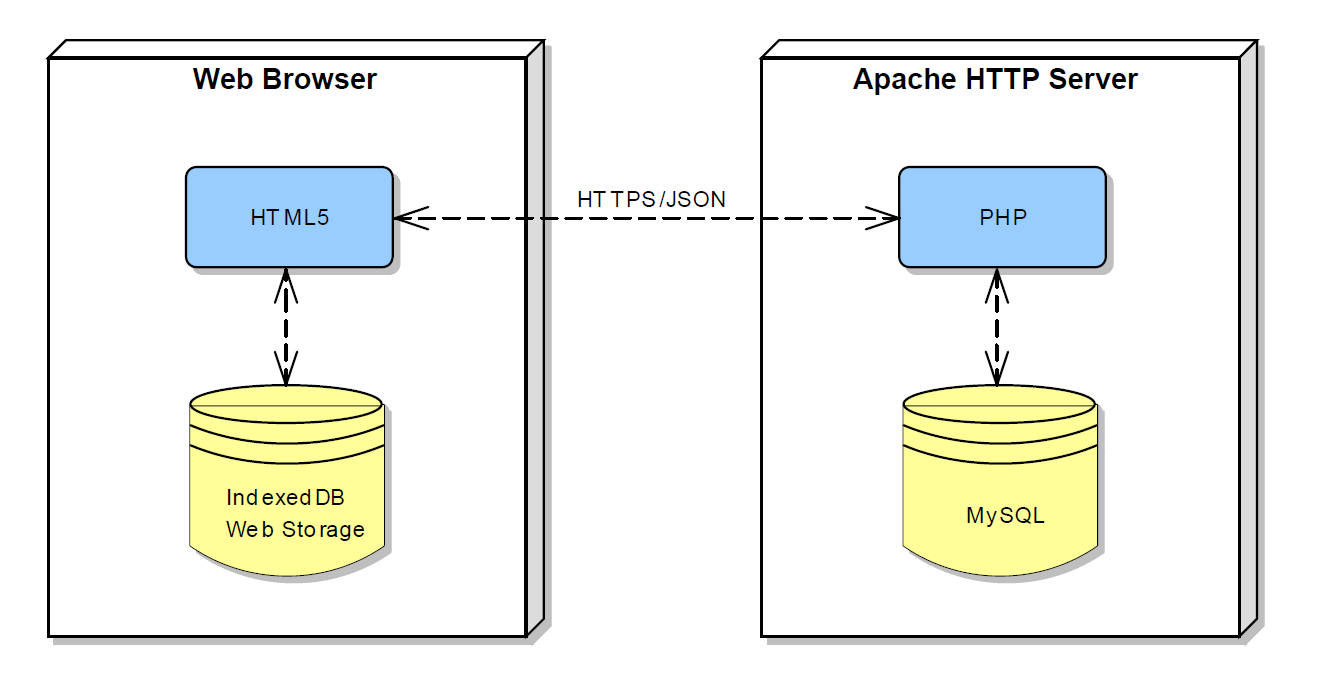
\includegraphics[width=1.0\textwidth]{architecture.png}
\caption{Uproszczony schemat architektury klient-serwer.}
\end{figure}

\subsection{Założenia}
\label{sec:zalozenia}

Podstawowym założeniem dotyczącym architektury aplikacji OffCalendar jest podział na część serwerową, której zadaniem będzie przyjmowanie i odpowiadanie na żądania napływające z aplikacji www, która stanowić ma część kliencką. Celem usprawnienia komunikacji i minimalizacji rozmiaru danych przesyłanych pomiędzy klientem i serwerem zdecydowano się na architekturę REST.

Dane zgromadzone za pomocą interfejsu użytkownika i przekonwertowane na lekki format JSON winny trafić do interfejsów serwera. Następnie odpowiednie moduły logiki systemu wykonają operacje CRUD (Create/Read/Update/Delete) i zwrócą rezultaty owych operacji z powrotem do aplikacji klienckiej, która dokona interpretacji zwróconych danych i odpowiednio zaprezentuje wyniki (aktualizacja widoku wydarzeń, komunikaty o błędach lub poprawnie zakończonych operacjach etc.).

Warunkiem koniecznym funkcjonowania komunikacji pomiędzy klientem i serwerem jest dostęp do sieci Internet. Jednocześnie aplikacja kliencka musi oferować wsparcie dla trybu offline. Będzie to możliwe z uwagi na fakt, że na serwerze spoczywa wyłącznie ciężar autoryzacji i synchronizacji danych. Dzięki zastosowaniu przechowywania lokalnego manipulacja danymi użytkownika odbywać się będzie z udziałem pamięci podręcznej przeglądarki. W sytuacji detekcji przejścia w tryb online zgromadzone dane winny zostać przesłane do serwera, gdzie nastąpi ich synchronizacja. Odbywać się to będzie co określony w systemie czas.

\subsection{Representational State Transfer (REST)}
\label{sec:REST}

REST \emph{(Representational State Transfer)}\cite{restTut} to oparty na bezstanowym protokole komunikacyjnym (w praktycznie wszystkich przypadkach jest używany protokół HTTP) styl architektoniczny służący projektowaniu aplikacji internetowych. Jego główne założenia, to:

\begin{itemize}
\item architektura klient-serwer,
\item bezstanowość (cache),
\item buforowanie podręczne,
\item jednolity interfejs dostępu.
\end{itemize}

Architektura REST opiera się na zasobach. Zasoby, czyli dane udostępnione przez system ''na zewnątrz'' są jednoznacznie indentyfikowane za pomocą adresu URL. Mogą one być reprezentowane z wykorzystaniem różnych formatów (JSON, XML etc.). Na potrzeby aplikacji OffCalendar wykorzystano format JSON z uwagi na prostotę i lekkość, co sprzyja wydajnej komunikacji bez zbędnych narzutów.

Na zasobach wykonywane są podstawowe operacje CRUD, odwzorowane w architekturze REST w następujący sposób:

\begin{enumerate}
\item\textbf{POST} - tworzenie
\item \textbf{GET} - odczyt
\item \textbf{PUT} - aktualizacja
\item \textbf{DELETE} - usuwanie.
\end{enumerate}

Tablica 3.1 przybliża przykładowe żądania z wykorzystaniem w/w metod\cite{rest2}:

\begin{table}[h]
\centering
    \begin{tabular}{ | p{7cm} | p{7cm} | }
    \hline
    \textbf{Przykładowa operacja} & \textbf{Żądanie REST} \\ \hline
	utwórz nowego użytkownika & \url{/app/users_api} \textbf{POST}
	\\ \hline
	wyświetl istniejących użytkowników & \url{/app/users_api} \textbf{GET}
	\\ \hline
	aktualizuj dane użytkownika & \url{/app/users_api/123} \textbf{PUT}
	\\ \hline
	usuń użytkownika & \url{/app/users_api/123} \textbf{DELETE}
	\\ \hline
    \end{tabular}
	\caption{Przykłady operacji i ich odwzorowania na żądania w architekturze REST.}
\end{table}

Każde żądanie kierowane do serwera jest niezależne od innych i nie można pomiędzy nimi znaleźć powiązań. Z uwagi na brak dodatkowych narzutów związanych ze standardami (np. SOAP) i prostotę implementacji REST stanowić będzie podstawę komunikacji w aplikacji OffCalendar\cite{rest3}\cite{rest4}.

\section{Aplikacja kliencka}
\label{sec:appKliencka}

Zadaniem aplikacji klienckiej będzie lokalne gromadzenie informacji użytkownika, detekcja trybu offline/online oraz komunikacja z aplikacją serwerową celem przeprowadzania autoryzacji oraz synchronizacji wydarzeń.

\subsection{Tryb offline}
\label{trybOff}

Wsparcie dla trybu offline w aplikacji OffCalendar realizowane będzie za pomocą metod lokalnego przechowywania danych oferowanych w ramach HTML5. Użytkownik nie dysponujący aktywnym połączeniem sieciowym nadal winien mieć możliwość wprowadzania/edytowania oraz usuwania wydarzeń. Zostaną one zapisane w pamięci podręcznej przeglądarki i podlegać będą bezproblemowemu dostępowi bez angażowania strony serwerowej.

Wykrywanie stanu połączenia internetowego odbywać się winno poprzez wykonanie żądania załadowania małego (110 bajtów) zasobu graficznego. Nieudana próba dostępu do pliku warunkuje przejście w tryb offline. Skutkuje to zawieszeniem wszystkich operacji angażujących stronę serwerową, a więc synchronizacji danych.
	
Istotną kwestię stanowi bezpieczeństwo aplikacji klienckiej. Z uwagi na fakt, iż to serwer odpowiadać ma za autoryzację użytkownika, a w trybie offline dostęp do niego nie będzie możliwy, pojawiające się niedogodności uwzględniono w konstrukcji interfejsu graficznego OffCalendar. Opierać się będzie on na jednym głównym widoku tzw. dashboard (przestrzeń robocza). Poszczególne jego sekcje będą ładowane asynchronicznie, co eliminuje konieczność weryfikacji praw użytkownika w trakcie przechodzenia pomiędzy widokami aplikacji. Wszystkie konieczne dane winny być pobierane przy pierwszym logowaniu i pozostaną do dyspozycji użytkownika do momentu wylogowania się.

\subsection{Tryb online}
\label{trybOn}

Praca aplikacji w trybie online obejmuje wykonywanie operacji wymagających komunikacji z serwerem. Składać się na nie będą:

\begin{itemize}
\item logowanie,
\item sprawdzenie, czy użytkownik posiada autoryzację,
\item tworzenie nowego konta,
\item synchronizacja wydarzeń z aplikacją serwerową.
\end{itemize}

Wyżej wymienione czynności winny być realizowane w oparciu o dane wprowadzane przez użytkowników i przechowywane lokalnie. Będzie to poprzedzone sprawdzeniem stanu połączenia internetowego. Przełączanie między trybami offline/online wykonywać się będzie automatycznie. W wypadku braku połączenia regularna synchronizacja zostanie zawieszona aż do momentu ponownego jego nawiązania.

\section{Aplikacja serwerowa}
\label{sec:appSerw}

Aplikacja serwerowa odpowiadać będzie za dostarczanie wymaganych przez aplikację kliencką zasobów, zarządzanie kontami użytkowników oraz wysyłanie notyfikacji o nadchodzących wydarzeniach.

Ze względu na duży nacisk kładziony na działanie aplikacji w trybie offline, szczególnie ważnym zadaniem spoczywającym na aplikacji serwerowej będzie wydajna synchronizacja wydarzeń pomiędzy aplikacjami klienckimi użytkowników.

\subsection{Warstwa danych}
\label{warstwaDanych}

Głównym zadaniem warstwy danych jest przechowywanie informacji o kontach użytkowników oraz wydarzeniach. Warstwa danych powinna udostępniać metody pozwalające na wydajne przeszukiwanie zbioru przechowywanych rekordów. Do tego celu na poszczególnych kolumnach powinny zostać zastosowane indeksy. 

Warstwa danych powinna również zapewnić konwersję rekordów pobranych z bazy danych do odpowiadających im klas, których założenia zostały przedstawione poniżej.

\textbf{Użytkownik (User)}

Dane użytkownika powinny zawierać:

\begin{itemize}
\item unikalny identyfikator użytkownika,
\item nazwę,
\item adres e-mail,
\item hasło.
\end{itemize}

Ze względu na bezpieczeństwo i poufność haseł użytkowników, powinny być one szyfrowane przed zapisem w bazie danych. Pozwoli to uchronić użytkowników przed nieautoryzowanym dostępem do kont w wyniku wycieku bazy danych.

\textbf{Wydarzenie (Event)}

Podstawowe własności wydarzenia to:

\begin{itemize}
\item unikalny identyfikator wydarzenia,
\item identyfikator użytkownika,
\item data rozpoczęcia,
\item data zakończenia,
\item opis.
\end{itemize}

Dodatkowo każde wydarzenie powinno posiadać pola stwierdzające konieczność wysłania powiadomienia e-mail oraz pole statusu wydarzenia (aktywne lub usunięte). 

Ze względu na konieczność synchronizacji danych, wydarzenie powinno posiadać stemple czasowe określające moment ostatniej aktualizacji danych, zarówno po stronie aplikacji klienckiej jak i serwerowej.

\subsection{Bezstanowe interfejsy}
\label{bezstanoweInter}

Aplikacja serwerowa będzie posiadać następujące interfejsy programowania aplikacji (API):

\begin{enumerate}
\item \textbf{UsersAPI} - interfejs zarządzania użytkownikami
\item \textbf{EventsAPI} - interfejs zarządzania wydarzeniami
\end{enumerate}

Interfejsy użytkownika są szczególnie ważnym elementem aplikacji OffCalendar ze względu na to, że są one jedyną formą pozyskania oraz aktualizacji danych. 

Aby zapewnić prywatność danych i bezpieczeństwo aplikacji, interfejsy powinny komunikować się z aplikacją kliencką za pośrednictwem protokołu HTTPS\cite{https}.

W przypadku pomyślnego przetworzenia żądania, interfejsy powinny zwracać odpowiednie dla danej metody dane zwrotne. W przeciwnym przypadku, powinien zostać zwrócony odpowiedni kod statusu oraz wiadomość zawierająca informację o błędach.

\textbf{UsersAPI}

UsersAPI to interfejs udostępniający metody tworzenia, modyfikacji i usuwania kont użytkowników aplikacji OffCalendar.

Dla metod innych niż tworzenie nowego konta konieczne jest przesłanie danych pozwalających na poprawną autentykację użytkownika. W przeciwnym wypadku żądanie powinno zostać odwołane.

\textbf{EventsAPI}

EventsAPI to interfejs udostępniający metody odpowiedzialne za synchronizację wydarzeń pomiędzy aplikacjami klienckimi użytkownika.

Ze względu na znaczną ilość przesyłanych danych, zarówno dane wejściowe, zawierające wydarzenia przechowywane po stronie klienta, jak i dane wyjściowe, zawierające zestaw wydarzeń wymagających aktualizacji, powinny być przesyłane w formacie JSON.

\subsection{Synchronizacja danych}
\label{synDanych}

Najważniejszym zadaniem aplikacji serwerowej jest synchronizacja danych pomiędzy aplikacjami klienckimi użytkowników.

Proces synchronizacji powinien być inicjowany przez aplikację kliencką, która do odpowiedniej metody interfejsu UsersAPI powinna przesłać:

\begin{itemize}
\item dane potrzebne do autentykacji użytkownika,
\item datę ostatniej synchronizacji,
\item wydarzenia zmodyfikowane po dacie ostatniej synchronizacji.
\end{itemize}

W przypadku pozytywnej autentykacji użytkownika, serwer powinien pobrać listę wszystkich wydarzeń zmodyfikowanych później niż przesłana data ostatniej synchronizacji. Następnie wydarzenia przesłane do serwera powinny zostać podzielone na trzy kategorie. W zależności od kategorii atrybuty wydarzeń będą modyfikowane w taki sposób, aby po zakończeniu procesu synchronizacji na serwerze i otrzymaniu przez aplikację kliencką wydarzeń zwrotnych, mogła ona zaktualizować dane przechowywane lokalnie. Wydarzenia powinny zostać skategoryzowane według poniższych kryteriów:

\begin{enumerate}
  \item Nowe wydarzenia - wydarzenia przesłane do aplikacji serwerowej po raz pierwszy. Powinny zostać dodane do bazy danych otrzymując tym samym ich unikalne identyfikatory, które zostaną dodane do atrybutów wydarzeń.
  \item Wydarzenia znajdujące się w bazie danych:
  \begin{itemize}
    \item Zaktualizowane później (nowsze) niż wydarzenia przechowywane w bazie danych. Poszczególne wydarzenia w bazie danych zostają zaktualizowane.
    \item Zaktualizowane wcześniej (starsze) niż wydarzenia przechowywane w bazie danych. Wydarzenia w bazie danych pozostają bez zmian.
  \end{itemize}
\end{enumerate}

We wszystkich trzech przypadkach modyfikowana jest również data ostatniej synchronizacji wydarzenia. W przypadku nowych wydarzeń oraz wydarzeń nowszych niż przechowywane w bazie jest to obecna data. W przypadku wydarzeń starszych jest to data aktualizacji danego wydarzenia.

Jeśli z bazy danych zostaną zwrócone wydarzenia które nie zostaną dopasowane do żadnego z wydarzeń przesłanych przez aplikację kliencką, wydarzenia te powinny zostać dołączone do listy zwracanych wydarzeń.

W odpowiedzi na żądanie synchronizacji, do aplikacji klienckiej powinien zostać zwrócony pełen zestaw wydarzeń zwrotnych oraz stempel czasowy synchronizacji. Na aplikacji klienckiej spoczywa ciężar aktualizacji wydarzeń przechowywanych w lokalnej bazie danych oraz zapis zwróconego stempla czasowego celem jego wykorzystania przy następnym procesie synchronizacji.